% Standalone Overleaf source: upload this file only and choose pdfLaTeX.
% All sections, bibliography, tables and figure coordinates are embedded.
% Repository maintenance: scripts/update_supplement.py replaces only GENERATED blocks.
\documentclass[11pt,a4paper]{article}
\usepackage[T1]{fontenc}
\usepackage[utf8]{inputenc}
\usepackage[margin=24mm]{geometry}
\usepackage{lmodern}
\usepackage{amsmath,amssymb}
\usepackage{booktabs,longtable,tabularx,array}
\usepackage{xcolor,listings,caption,fancyhdr,microtype}
\usepackage{tikz,pgfplots}
\usetikzlibrary{arrows.meta,positioning,fit}
\pgfplotsset{compat=1.18}
\usepackage{xurl}
\usepackage[colorlinks=true,linkcolor=blue!50!black,citecolor=blue!50!black,urlcolor=blue!50!black]{hyperref}
% BEGIN GENERATED: metadata
\newcommand{\PackageVersion}{0.2.0}
\newcommand{\SnapshotHash}{81caa5c55054d278836b1a072952cb61ff9567953c6aa293244058c475dd8102}
\newcommand{\PaperHash}{30fcc98b7d9191c0f5b5fe909b817d09138dddafb0877010853901daf25126fd}
\newcommand{\MigrationChecks}{22}
\newcommand{\OriginalAuditPassed}{80}
\newcommand{\BootstrapCount}{100}
\newcommand{\BootstrapCoverage}{1.000}
\newcommand{\BootstrapWidth}{0.240408}
\newcommand{\RecordedPython}{3.12.3}
\newcommand{\RecordedNumpy}{2.4.6}
\newcommand{\RecordedScipy}{1.18.1}
% END GENERATED: metadata
\hypersetup{pdftitle={Supplementary material: software structure and reproducibility for Hx-NdNiO3 reduced models},pdfauthor={Companion computational documentation}}
\newcommand{\material}{\ensuremath{\mathrm{H}_x\text{--}\mathrm{NdNiO}_3}}
\newcommand{\code}[1]{\texttt{\detokenize{#1}}}
\newcommand{\repo}[1]{\path{#1}}
\renewcommand{\thesection}{S\arabic{section}}
\renewcommand{\thetable}{S\arabic{table}}
\renewcommand{\thefigure}{S\arabic{figure}}
\renewcommand{\theequation}{S\arabic{equation}}
\setcounter{tocdepth}{2}
\setlength{\parskip}{4pt}
\setlength{\parindent}{0pt}
\setlength{\headheight}{14pt}
\setlength{\emergencystretch}{2em}
\pagestyle{fancy}\fancyhf{}
\fancyhead[L]{\small Supplementary software documentation}
\fancyhead[R]{\small OgTRQC / \PackageVersion}
\fancyfoot[C]{\thepage}
\lstset{basicstyle=\small\ttfamily,breaklines=true,columns=fullflexible,keepspaces=true,
 frame=single,rulecolor=\color{black!20},backgroundcolor=\color{black!2},showstringspaces=false,
 xleftmargin=3pt,xrightmargin=3pt}
\captionsetup{font=small,labelfont=bf}
\title{Supplementary Material\\[5pt]\large Software structure, scientific correspondence, and computational reproducibility for\\[4pt]
\textit{Proton Transport and Polarization Relaxation in \material: Literature-Constrained Reduced Models and a Recoverability Diagnostic}}
\author{Companion documentation for the OgTRQC repository}
\date{Package version \PackageVersion\quad---\quad Working-tree implementation snapshot}
\begin{document}
\maketitle
\begin{abstract}
This supplement documents the relationship between the manuscript's reduced models and the accompanying software. It identifies the object-oriented implementation, the unchanged original notebook record, and the historical quantum-geometric prototypes as distinct software categories. It specifies state conventions, physical units, parameter transfer, calibration partitions, numerical protocols, and recorded verification. Numerical tables and plot coordinates are embedded from the repository's recorded CSV and JSON results; compiling this document does not refit models. Experimental holdout evaluation is distinguished from migration fidelity, frozen-generator checks, and synthetic state-sufficiency experiments. The software does not supply a dynamically calibrated concentration-to-polarization map, a general nonlinear transport solver, or independent microscopic parameter identification. This file is self-contained and can be compiled directly in Overleaf using pdfLaTeX.
\end{abstract}
\tableofcontents
\clearpage

\section{Scope and implementation categories}\label{sec:scope}

The companion manuscript~\cite{manuscript} separates three components: a structure-conditioned spatial transport model, an independently fitted polarization-relaxation model, and a recoverability diagnostic. The current software reproduces this separation in the namespace \repo{octa_gtrqc_sim.proton}. Its primary entry point is \code{proton-study}. The archived computational record is executed independently through \code{proton-reference}. Both commands are installed by Poetry.

The repository also preserves earlier quantum-geometric prototypes. These use different state representations and, in some engines, drive geometry using a recoverability loss. They are historical development artifacts, not alternative numerical realizations of the present paper. A scientific claim about the current manuscript must therefore identify the current namespace or the original reference notebook, rather than referring to every file in the repository indiscriminately.

\subsection{Directory boundaries and compatibility}

\begin{longtable}{@{}p{.38\linewidth}p{.57\linewidth}@{}}
\caption{Repository categories and their scientific roles.}\label{tab:layout}\\
\toprule Location & Role and interpretation\\\midrule\endfirsthead
\toprule Location & Role and interpretation\\\midrule\endhead
\repo{octa_gtrqc_sim/proton/} & Current object-oriented physical models, inference protocols, diagnostics and MVP orchestration.\\
\repo{notebooks/reference/} & Four unchanged original notebooks, with a SHA-256 manifest. This is the complete original computational record.\\
\repo{notebooks/paper_workflow.ipynb} & Small interactive client of the current API. It is not the complete experimental or synthetic validation campaign.\\
\repo{validation/native/} & Recorded outputs from the native package: tables, metadata, arrays, vector figures and artifact manifests.\\
\repo{validation/reference/} & Compact records of original notebook executions and their outputs.\\
\repo{validation/migration.json} & Explicit numerical comparisons between native and reference calculations, including tolerances.\\
Top-level Python modules in \repo{octa_gtrqc_sim/}, outside \repo{proton/} & Historical engines and compatibility entry points. They are excluded from the current paper's physical interpretation.\\
\repo{reports_*/}, \repo{robustness_reports/} & Historical delay, Hilbert-dimension and sensitivity reports. Their existence does not provide validation for the current paper.\\
\repo{docs/source/} & Sphinx source for the current API and explicitly labelled historical documentation.\\
\repo{supplementary/main.tex} & This self-contained document, including its numerical figures and bibliography.\\
\bottomrule
\end{longtable}

The current implementation already occupies a separate physical directory. Historical modules retain their original import paths so that previous scripts continue to work. Their physical relocation into a new legacy namespace is not required for the present scientific separation and has not been performed. The repository-level \repo{VARIANTS.md} records this policy. New paper-related code belongs in the current namespace, and original notebook sources remain unchanged.

\subsection{Native coverage versus full reference execution}

The distinction between a reusable API and a complete original computation is important. Core structural and transport laws, polarization fitting, uncertainty, parameter profiles, and the review generator audits have native class-based implementations. The larger synthetic risk, distribution-shift and hidden-twin sensor-selection experiments remain available through original notebook replay. The native \code{hidden_state} command is a deterministic reflected-profile illustration; its output must not be substituted for the original ROC-AUC, protocol-transfer or sensor-selection results.

\begin{longtable}{@{}p{.19\linewidth}p{.34\linewidth}p{.40\linewidth}@{}}
\caption{Manuscript-to-software correspondence. Section numbers refer to the supplied manuscript~\cite{manuscript}.}\label{tab:correspondence}\\
\toprule Manuscript & Native implementation & Scope or full reference route\\\midrule\endfirsthead
\toprule Manuscript & Native implementation & Scope or full reference route\\\midrule\endhead
Sections 2.3, 2.6 & \code{RecoverabilityDiagnostic} & Bernoulli mean-projection diagnostic; exactly absent from physical forces and hopping rates.\\
Sections 2.4--2.5 & \code{StructuralModel} & Two-mode energy, equilibrium and forces. Broader mode-basis, strain-prior and structural sensitivity analyses remain in v3.1 replay.\\
Section 2.7 & \code{TransportModel}, \code{FrozenGenerator} & Structure-conditioned generator and frozen probability propagation. No general nonlinear self-consistent occupancy solver is claimed.\\
Section 2.8; Results 3.1--3.3 & \code{RelaxationModel}, \code{CalibrationStudy} & Independent field-law models, strict holdout, retrospective field folds and working information criteria.\\
Section 2.10; Result 3.6 & \code{ContinuumStudy}, \code{RefinementStudy} & Constant-$D$ benchmark and distinct R3 full-generator refinement, respectively.\\
Section 2.14; Result 3.4 & \code{IdentifiabilityStudy}; calibration bootstrap & Original alpha grid, five additional nuisance profiles and pointwise predictive uncertainty.\\
Section 2.7; Result 3.5 & \code{TransportSensitivityStudy} & Independent transport-coefficient sweep and frozen-generator checks.\\
Sections 2.9, 2.11; Results 3.7--3.8 & Full v3.1 reference notebook & Vacancy measurement-rank illustration, synthetic risk/transfer ensembles and prospective hidden-twin sensor design.\\
Section 2.12 & No dedicated native inverse solver & Optional inverse-observation discussion is not presented as implemented material evidence.\\
Result 3.9 & Original notebook audit and migration record & Original 80-gate audit is distinct from unit tests and migration comparisons.\\
\bottomrule
\end{longtable}

\section{Object-oriented architecture and execution flow}\label{sec:architecture}

The software follows Model--View--Presenter (MVP), the architectural pattern of the repository. MVP here refers to software separation of concerns, not to Model Context Protocol. The implementation provides a Python API and CLI; no MCP server is required for reproduction.

\subsection{Model and study layer}

\code{StructuralModel} stores the calibrated two-mode priors. \code{DeviceConfig} stores geometry, temperature, field, diffusivity and the explicit transport coefficient. \code{TransportModel.freeze} constructs a \code{FrozenGenerator}, which exposes the column generator, its stationary distribution, probability propagation and physical audits. \code{RelaxationModel} owns prediction laws, optimizer bounds and initializations. \code{FitResult} records the calibration indices, optimizer result and local covariance. \code{PolarizationDataset} validates and loads the offline experimental matrix.

Studies compose these models into reproducible numerical protocols. They return a \code{StudyResult} containing named tables, metadata and optional arrays. The numerical models do not write reports or invoke a user interface. Recoverability is implemented independently and supplies no argument to the physical force or rate laws.

\subsection{Presenter and view layer}

\code{PaperPresenter} dispatches a named study and passes its result to the \code{StudyView} protocol. \code{ArtifactView} writes CSV, JSON, NPZ, Markdown and available PDF/SVG figures. It then records a SHA-256 manifest for the produced artifacts. A new view can therefore be added without modifying the scientific laws.

\begin{figure}[htbp]
\centering
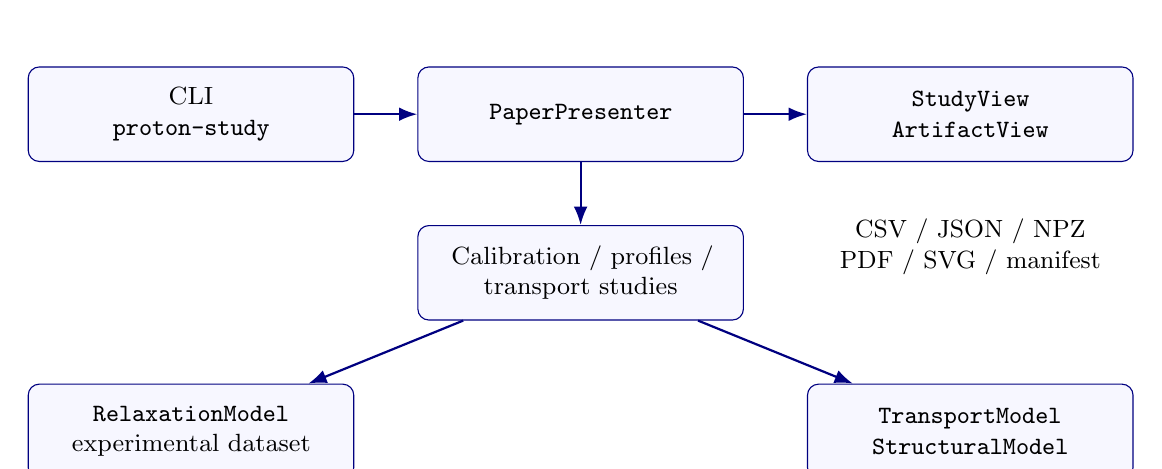
\begin{tikzpicture}[>=Latex,node distance=8mm and 8mm,
 box/.style={draw=blue!50!black,rounded corners,fill=blue!3,align=center,font=\small,text width=39mm,minimum height=12mm},
 arrow/.style={->,thick,draw=blue!50!black}]
\node[box] (cli) {CLI\\\texttt{proton-study}};
\node[box,right=of cli] (presenter) {\texttt{PaperPresenter}};
\node[box,right=of presenter] (view) {\texttt{StudyView}\\\texttt{ArtifactView}};
\node[box,below=of presenter] (study) {Calibration / profiles /\\transport studies};
\node[box,below left=of study] (relax) {\texttt{RelaxationModel}\\experimental dataset};
\node[box,below right=of study] (transport) {\texttt{TransportModel}\\\texttt{StructuralModel}};
\draw[arrow] (cli)--(presenter);
\draw[arrow] (presenter)--(study);
\draw[arrow] (study)--(relax);
\draw[arrow] (study)--(transport);
\draw[arrow] (presenter)--(view);
\node[font=\small,align=center,below=6mm of view] {CSV / JSON / NPZ\\PDF / SVG / manifest};
\end{tikzpicture}
\caption{MVP responsibilities. Studies return presentation-neutral results. The presenter coordinates execution and reporting; the view does not fit or select a scientific model. The architecture is also documented through Mermaid UML diagrams in the repository README and Sphinx pages.}
\label{fig:architecture}
\end{figure}

\subsection{Independent reference adapter}

\code{ReferenceNotebookRunner} verifies each archived notebook against its manifest, starts the Poetry interpreter as a Jupyter kernel, and executes the notebook in a separate output directory. Source notebooks are not edited. The v3.1 executed copy receives a final export cell that serializes the completed summary and pandas tables; this cell is not inserted into the archived source. Execution failure propagates, and the partially executed copy and status record are retained. Native model imports do not execute notebook source.

\section{Scientific state, units and physical laws}\label{sec:physics}

\subsection{Geometry and state representation}

A one-dimensional device interval of length $L$ is divided into $N$ coarse cells of width $h=L/N$, with centres $x_i=(i+1/2)h$ for zero-based index $i$. A cell represents a material volume containing local coordination environments. It is not an oxygen vertex, an atomistically resolved octahedron, or a complete crystallographic unit cell. Mean proton occupancy is denoted $c_i\in[0,1]$, with donated-electron bookkeeping $n_i^e=c_i$.

Three objects must be distinguished: the local radial cage coordinate, the retained staggered-order proxy, and the device mesh. The current transport API treats the occupancy background as prescribed when constructing a generator. Its propagator then evolves a normalized probability $p$, not a guaranteed saturation-respecting nonlinear occupancy field. Although the manuscript writes a formal state-dependent transport law, the reported frozen checks do not constitute a numerical solution or stability theorem for that full nonlinear problem.

\subsection{Structural free energy and calibrated priors}

For the two retained coordinates, the implemented structural free energy is
\begin{equation}
 F_{\rm str}=\sum_{i=0}^{N-1}\left(\frac12K_A Q_{A,i}^2-g_A c_iQ_{A,i}\right)
 +N\left(\frac12K_RQ_R^2-g_Rm_{\pi,N}Q_R\right),
 \label{eq:energy}
\end{equation}
where
\begin{equation}
 m_{\pi,N}=\frac{\left|\sum_i(-1)^ic_i\right|}{\sum_i c_i},\qquad
 g_A=K_AQ_A^{(1)},\qquad g_R=K_RQ_R^{\rm bulk}.
\end{equation}
An empty proton configuration has zero order. The implementation regularizes the mass denominator by $10^{-15}$. The transport construction additionally clips validated occupancies to $[10^{-12},1-10^{-12}]$ to retain the original notebook's rate convention.

The exact harmonic minimizers are $Q_{A,i}^*=Q_A^{(1)}c_i$ and $Q_R^*=Q_R^{\rm bulk}m_{\pi,N}$. The returned forces are $-K_A(Q_{A,i}-Q_{A,i}^*)$ and $-K_R(Q_R-Q_R^*)$, with the latter expressed per cell. Native transport uses this adiabatic closure; it does not integrate a separate structural relaxation timescale.

\begin{table}[htbp]
\centering\small
\caption{Default priors and numerical conventions. Values are taken from the declared model and supplied notebook record, not independently inferred from the polarization holdout.}\label{tab:parameters}
\begin{tabular}{@{}lll@{}}\toprule
Quantity & Value & Unit or role\\\midrule
Reference Ni--O distance & 1.942 & \AA\\
Local volume expansion & 0.12 & Fraction at unit occupancy\\
Effective cage frequency & 420 & cm$^{-1}$\\
$K_A$ & 10.3784205761 & eV\,\AA$^{-2}$\\
$Q_A^{(1)}$ & 0.1831353882 & \AA\\
$E_A=K_A(Q_A^{(1)})^2/2$ & 0.1740386946 & eV\\
$K_R$ & 36.6666666667 & eV\,\AA$^{-2}$\\
$Q_R^{\rm bulk}$ & 0.06 & \AA\\
$E_R=K_R(Q_R^{\rm bulk})^2/2$ & 0.066 & eV per formula unit\\
$L$, $T$, $E$ & $10^{-7}$, 300, $2\times10^5$ & m, K, V/m\\
$D_{\rm rep}$ & $1.3416407865\times10^{-18}$ & m$^2$/s\\
$E_m$ & 0.41 & eV\\
Nominal $\chi_A^{\rm tr}$ & 0.9698094586 & Conditional transferred coefficient\\
Strain $\varepsilon$ & 0 & Dimensionless; configured range $\pm0.03$\\
\bottomrule\end{tabular}
\end{table}

The cage stiffness uses oxygen mass and the effective spectral prior; the breathing curvature uses the source convention cited in the manuscript~\cite{lione}. These are reduced structural scales. Positive definiteness of the retained $2\times2$ block establishes harmonic stability only within that subspace. The native module does not assign stiffnesses to omitted tilts, rotations, polar coordinates or Jahn--Teller modes.

\subsection{Structure-conditioned local-detailed-balance generator}

The reference diffusivity changes with temperature according to
\begin{equation}
 D_{\rm ref}(T)=D_{\rm rep}\exp\left[-\frac{E_m}{k_B}\left(\frac1T-\frac1{300\,\mathrm K}\right)\right].
\end{equation}
With $k_B$ expressed in eV/K, the site energy and edge barrier are
\begin{align}
 U_i &=-Ex_i-0.20E_A\frac{Q_{A,i}}{Q_A^{(1)}}
       -0.10E_R\frac{Q_R}{Q_R^{\rm bulk}}(-1)^i,\\
 B_{i+1/2} &=\chi_A^{\rm tr}E_A\frac{Q_{A,i}+Q_{A,i+1}}{2Q_A^{(1)}}
       +0.20E_R\frac{Q_R}{Q_R^{\rm bulk}}
       +0.15E_A\frac{\varepsilon}{0.01},\\
 D_{i+1/2}&=D_{\rm ref}(T)\exp[-B_{i+1/2}/(k_BT)].
\end{align}
$Q_R$ is nonnegative under the absolute-order convention, so its signed and absolute values coincide here. The electric contribution $-Ex_i$ is in eV for a singly charged proton when $E$ is in V/m and $x_i$ in m. The fixed numerical coefficients are declared reduced-model sensitivities, not separately measured constants.

Rates and matrix orientation are explicit:
\begin{align}
 k_i^+&=\frac{D_{i+1/2}}{h^2}\exp\left[-\frac{U_{i+1}-U_i}{2k_BT}\right],\quad
 k_i^-=\frac{D_{i+1/2}}{h^2}\exp\left[+\frac{U_{i+1}-U_i}{2k_BT}\right],\\
 Q_{i+1,i}&=k_i^+,\qquad Q_{i,i+1}=k_i^-,\qquad
 Q_{ii}=-\sum_{j\ne i}Q_{ji},\qquad \dot p=Qp.
 \label{eq:generator}
\end{align}
Reflecting boundaries omit jumps outside the mesh. Consequently $\mathbf1^TQ=0$, off-diagonal entries are positive, and the stationary distribution is proportional to $\exp[-U_i/(k_BT)]$. The sparse propagator computes $\exp(tQ)p_0$ without clipping or renormalizing the output to conceal numerical mass errors. Its input is checked for nonnegativity, finite values and unit mass.

The default transport coefficient is the original notebook's nominal transferred value. Recomputing the polarization fit can change its last digits through optimizer roundoff; the transport API does not silently replace its configured coefficient. The user can supply a new \code{DeviceConfig} explicitly. The coefficient sweep therefore tests conditional transport sensitivity without changing the polarization fit.

\subsection{Recoverability remains diagnostic}

The classical specialization under projection to mean occupancy is
\begin{equation}
 \Delta(c)=\frac1N\sum_i\left[c_i\log\frac{c_i}{\bar c}
 +(1-c_i)\log\frac{1-c_i}{1-\bar c}\right],\qquad \bar c=\frac1N\sum_i c_i.
 \label{eq:recoverability}
\end{equation}
The returned unit is nats per site. The implementation uses the continuous endpoint convention and returns zero for uniform zero or unit occupancy. This diagnostic appears in neither Eq.~\eqref{eq:energy} nor Eq.~\eqref{eq:generator}. There is no recoverability-to-force or recoverability-to-rate feedback in the current namespace.

Reflected occupancy profiles have equal mean and recoverability but may have distinct directed future observations. The native illustration propagates a ramp and its reflection under the same field-only generator. The larger original risk and sensor-selection protocols remain in reference replay. A scalar diagnostic that flags lost information does not reconstruct the missing directed state.

\section{Experimental data and independent relaxation inference}\label{sec:inference}

\subsection{Offline data and calibration boundary}

The original notebook embeds an $87\times12$ numerical matrix from the publisher source data associated with Yuan et al.~\cite{yuan}. The package stores those numbers in \repo{data/fig2h.json}, inside the current namespace. \code{PolarizationDataset.load} checks the shape and SHA-256 of the contiguous little-endian float64 matrix before constructing the working dataset.

Using zero-based source columns, time is column 0 multiplied by $10^{-3}$ to convert milliseconds to seconds. The four observation columns are column 10 divided by its first value for 133 kV/cm, column 9 for 267 kV/cm, column 6 for 400 kV/cm, and column 3 for 533 kV/cm. The original clipping to $[0,1.2]$ is retained. Publisher fitted curves are not calibration targets for the native models.

Primary calibration uses $3\times87=261$ observations at 133, 267 and 400 kV/cm. All 87 observations at 533 kV/cm are reserved for the primary external field holdout. A unit test changes every holdout value and verifies that the fitted calibration parameters remain unchanged. This tests the implementation's data boundary, not a claim of independence between experimental time points.

\subsection{Distributed spectrum and comparator models}

Let $f=(E_{\mathrm{kV/cm}}-333)/200$ and $z_j=j/20$, $j=0,\ldots,20$. The independent phenomenological readout is
\begin{align}
 P(t;f)&=\sum_{j=0}^{20}w_j(f)\exp[-t/\tau_j(f)],\\
 \log\tau_j&=\ell_0+\alpha_Az_j+c_Ff,\qquad
 \alpha_A=\chi_A^{\rm cond}\frac{E_A}{k_BT_{\rm fit}},\\
 w_j(f)&=\frac{\exp[(b_0+b_1f)z_j+b_2(z_j-1/2)^2]}
 {\sum_k\exp[(b_0+b_1f)z_k+b_2(z_k-1/2)^2]}.
 \label{eq:relaxation}
\end{align}
The code optimizes $\psi=(\ell_0,\chi_A^{\rm cond},b_0,b_1,b_2,c_F)$ with $T_{\rm fit}=300$ K. A numerically stabilized softmax defines weights. The scale identified through this fit is $\alpha_A$; interpreting $\chi_A^{\rm cond}$ requires fixing $E_A$ and temperature. Transferring $\chi_A^{\rm cond}$ to $\chi_A^{\rm tr}$ is a declared hypothesis, not a separately validated common mechanism.

The single exponential has a log-linear field dependence of its time constant and two parameters. The stretched exponential adds a field-dependent exponent constrained by $0.05+0.90\,\mathrm{logistic}(\cdot)$, giving four parameters. The retrospective biexponential uses two log-linear time constants and a logistic mixture weight, giving six parameters.

For the distributed spectrum, bounds are
\begin{equation}
 (\log10^{-6},0.05,-20,-20,-20,-5)\leq\psi
 \leq(0,3,20,20,20,5),
\end{equation}
with initial value $(\log(7\times10^{-4}),1,0,0,0,1)$. The original distributed fit uses SciPy \code{least_squares}, up to 20,000 function evaluations, and tolerances \code{xtol=ftol=gtol=1e-11}. The original single and stretched fits preserve their own initializations, budgets of 10,000 and 15,000 evaluations, and SciPy default tolerances. The biexponential uses three prescribed starts; selection is by training residual sum of squares only.

No transported concentration or probability trajectory is an input to Eq.~\eqref{eq:relaxation}. Removing the transport calculation would leave these fitted polarization predictions unchanged.

\subsection{Primary prediction and retrospective comparison}

\begin{table}[htbp]\centering\small
\caption{Recorded native evaluation on the complete 533 kV/cm holdout. Lag-one residual correlation is included to make the working independence assumption assessable.}
\label{tab:holdout}
% BEGIN GENERATED: holdout_table
\begin{tabular}{lrrrr}
\toprule
Model & Parameters & RMSE & $R^2$ & Lag-1 corr. \\
\midrule
Single exponential & 2 & 0.16117378 & 0.65569513 & 0.99372 \\
Stretched exponential & 4 & 0.04995229 & 0.96692764 & 0.95538 \\
Distributed spectrum & 6 & 0.02633725 & 0.99080620 & 0.81445 \\
\bottomrule
\end{tabular}
% END GENERATED: holdout_table
\end{table}

\begin{figure}[htbp]\centering
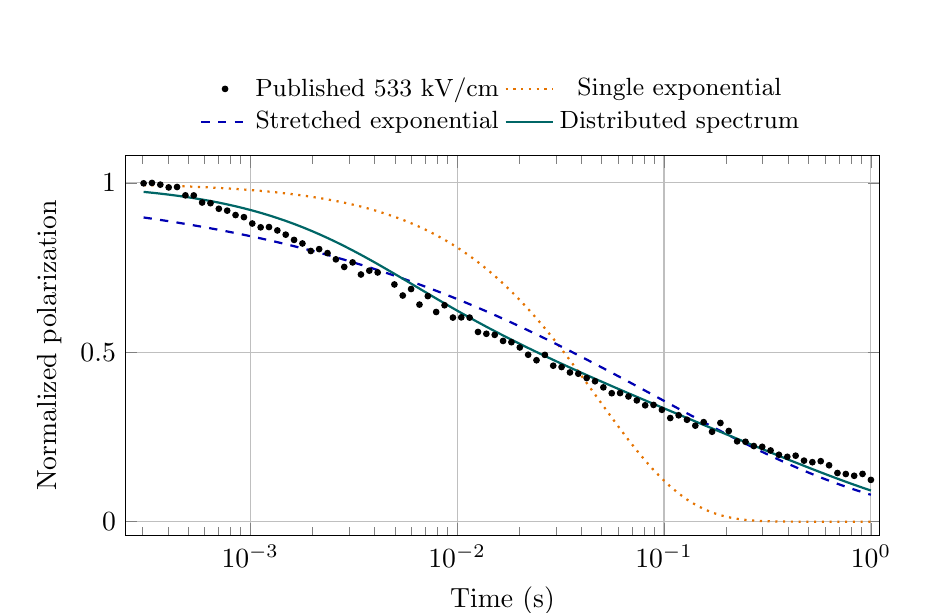
\begin{tikzpicture}
\begin{semilogxaxis}[width=.92\linewidth,height=64mm,xlabel={Time (s)},ylabel={Normalized polarization},
 xmin=0.00025,xmax=1.1,ymin=-.04,ymax=1.08,grid=major,
 legend style={font=\small,at={(.5,1.03)},anchor=south,legend columns=2,draw=none}]
% BEGIN GENERATED: holdout_plot
\addplot[only marks,mark=*,mark size=1.0pt,black] coordinates {
(0.00030539,0.99882) (0.00033516000000000004,1.0) (0.00036784000000000003,0.9949) (0.0004037,0.98685) (0.00044306,0.98799) (0.00048626,0.96335) (0.00053367,0.96316) (0.0005857,0.94221) (0.00064281,0.94022) (0.00070548,0.92379) (0.0007742599999999999,0.9182) (0.00084975,0.90521) (0.0009326,0.89902) (0.0010235300000000001,0.88021) (0.0011233200000000001,0.86898) (0.00123285,0.8697) (0.0013530500000000002,0.85976) (0.00148497,0.84735) (0.0016297500000000001,0.83184) (0.0017886500000000001,0.82131) (0.00196304,0.79909) (0.00215443,0.80459) (0.00236449,0.79284) (0.00259502,0.77442) (0.00284804,0.752) (0.00312572,0.76539) (0.00343047,0.72969) (0.00376494,0.74101) (0.00413201,0.73574) (0.00497702,0.7003) (0.00546228,0.66768) (0.00599484,0.68682) (0.0065793299999999996,0.64085) (0.00722081,0.66591) (0.00792483,0.61902) (0.00869749,0.63898) (0.00954548,0.60257) (0.01047616,0.60319) (0.01149757,0.60247) (0.01261857,0.56013) (0.013848860000000001,0.55473) (0.01519911,0.55152) (0.01668101,0.53359) (0.018307379999999998,0.52986) (0.020092330000000002,0.51435) (0.02205131,0.49282) (0.024201280000000002,0.47659) (0.026560880000000002,0.49246) (0.02915053,0.46052) (0.03199267,0.45653) (0.03511192,0.44059) (0.03853529000000001,0.43683) (0.042292430000000006,0.4241) (0.04641589,0.41448) (0.05094138,0.39652) (0.055908099999999995,0.37924) (0.06135907,0.37973) (0.06734151000000001,0.36969) (0.07390722,0.3581) (0.08111308,0.34361) (0.08902151000000001,0.34472) (0.097701,0.33029) (0.10722672,0.30601) (0.1176812,0.31409) (0.12915497,0.30084) (0.14174742,0.28356) (0.15556761,0.2939) (0.17073526000000003,0.26547) (0.18738174000000002,0.29148) (0.20565123,0.26786) (0.22570197,0.23723) (0.24770764,0.23592) (0.27185882,0.22329) (0.29836471999999997,0.22103) (0.32745492000000004,0.21033) (0.35938137000000003,0.19754) (0.39442061,0.19152) (0.43287613,0.19486) (0.47508102,0.18023) (0.52140083,0.17565) (0.57223677,0.17869) (0.62802914,0.16655) (0.6892612100000001,0.14375) (0.7564633300000001,0.14077) (0.8302175700000001,0.1355) (0.9111627600000001,0.14109) (1.0,0.12346)
};
\addlegendentry{Published 533 kV/cm}
\addplot[dotted,thick,orange!90!black] coordinates {
(0.00030539,0.993576174563284) (0.00033516000000000004,0.9929521794684856) (0.00036784000000000003,0.9922676404303993) (0.0004037,0.9915170338240591) (0.00044306,0.9906938202899571) (0.00048626,0.9897910799714931) (0.00053367,0.9888013109864087) (0.0005857,0.9877162302775685) (0.00064281,0.9865265774003561) (0.00070548,0.9852227535513651) (0.0007742599999999999,0.9837937969173889) (0.00084975,0.9822278205290439) (0.0009326,0.9805120360657147) (0.0010235300000000001,0.9786323683030469) (0.0011233200000000001,0.9765736971211547) (0.00123285,0.9743190743909838) (0.0013530500000000002,0.9718508049365673) (0.00148497,0.9691490655396523) (0.0016297500000000001,0.9661925956027979) (0.0017886500000000001,0.9629581693978211) (0.00196304,0.959420903519254) (0.00215443,0.9555537690513023) (0.00236449,0.9513273373725374) (0.00259502,0.9467105586454398) (0.00284804,0.9416691635443444) (0.00312572,0.9361673139190755) (0.00343047,0.9301661009876325) (0.00376494,0.9236239058929268) (0.00413201,0.9164970058415821) (0.00497702,0.900298905990553) (0.00546228,0.8911266314179451) (0.00599484,0.8811678216106243) (0.0065793299999999996,0.8703659828541755) (0.00722081,0.8586632735390021) (0.00792483,0.8460006595327119) (0.00869749,0.8323183031947954) (0.00954548,0.8175565570039975) (0.01047616,0.8016565244806988) (0.01149757,0.7845621218209463) (0.01261857,0.7662202437844224) (0.013848860000000001,0.746583330178738) (0.01519911,0.7256104836291204) (0.01668101,0.7032702822012058) (0.018307379999999998,0.6795430074421016) (0.020092330000000002,0.6544225857356837) (0.02205131,0.6279205044517977) (0.024201280000000002,0.6000682792298456) (0.026560880000000002,0.5709202697421946) (0.02915053,0.5405575007628405) (0.03199267,0.5090897102685539) (0.03511192,0.47665822237434435) (0.03853529000000001,0.44343775507573047) (0.042292430000000006,0.40963713245207234) (0.04641589,0.3754989497496336) (0.05094138,0.34129790365660484) (0.055908099999999995,0.307336924032206) (0.06135907,0.27394149199177303) (0.06734151000000001,0.2414516008977702) (0.07390722,0.21021166996415766) (0.08111308,0.18055799502990072) (0.08902151000000001,0.15280505710354267) (0.097701,0.1272307650492224) (0.10722672,0.10406172976185504) (0.1176812,0.08345993930794984) (0.12915497,0.0655124020035317) (0.14174742,0.05022460490654826) (0.15556761,0.03751954576526534) (0.17073526000000003,0.027242655880065414) (0.18738174000000002,0.019172916033787648) (0.20565123,0.013039242780081004) (0.22570197,0.00854066749339638) (0.24770764,0.005368027840393985) (0.27185882,0.003224590607206776) (0.29836471999999997,0.001843121335159764) (0.32745492000000004,0.0009975823009786594) (0.35938137000000003,0.0005085690725171047) (0.39442061,0.00024278571545858002) (0.43287613,0.00010784173645459522) (0.47508102,4.425766264959736e-05) (0.52140083,1.6652435205434515e-05) (0.57223677,5.696101340204659e-06) (0.62802914,1.7549028822628743e-06) (0.6892612100000001,4.820308463242259e-07) (0.7564633300000001,1.1672997652378681e-07) (0.8302175700000001,2.461734703893794e-08) (0.9111627600000001,4.4606345718571644e-09) (1.0,6.842631730738202e-10)
};
\addlegendentry{Single exponential}
\addplot[dashed,thick,blue!70!black] coordinates {
(0.00030539,0.8980598582907185) (0.00033516000000000004,0.8944968956780914) (0.00036784000000000003,0.890816257686785) (0.0004037,0.8870161643744734) (0.00044306,0.8830922867664629) (0.00048626,0.8790414145769975) (0.00053367,0.8748605457698055) (0.0005857,0.8705462672173715) (0.00064281,0.8660943691193256) (0.00070548,0.8615024865576236) (0.0007742599999999999,0.8567665143398999) (0.00084975,0.8518826389399455) (0.0009326,0.8468475751603967) (0.0010235300000000001,0.8416576250730727) (0.0011233200000000001,0.8363096417112209) (0.00123285,0.8307992557449605) (0.0013530500000000002,0.8251238769594145) (0.00148497,0.819279538880036) (0.0016297500000000001,0.8132628776929701) (0.0017886500000000001,0.8070702250971881) (0.00196304,0.8006984634605382) (0.00215443,0.7941442937060386) (0.00236449,0.7874041029575594) (0.00259502,0.7804753950513234) (0.00284804,0.773354475275321) (0.00312572,0.7660390854781385) (0.00343047,0.758526335303631) (0.00376494,0.750813409660748) (0.00413201,0.7428983077024616) (0.00497702,0.7264521226628964) (0.00546228,0.7179173716300371) (0.00599484,0.7091730981439626) (0.0065793299999999996,0.7002178425833055) (0.00722081,0.6910508038243882) (0.00792483,0.6816715528038891) (0.00869749,0.6720799017242867) (0.00954548,0.6622761110875767) (0.01047616,0.6522606690881533) (0.01149757,0.6420349015877912) (0.01261857,0.6316002400267701) (0.013848860000000001,0.620958839707926) (0.01519911,0.6101131797127394) (0.01668101,0.5990664637885599) (0.018307379999999998,0.587822535531999) (0.020092330000000002,0.5763855813411479) (0.02205131,0.564760661607786) (0.024201280000000002,0.5529534670087818) (0.026560880000000002,0.5409702388339352) (0.02915053,0.5288181183245907) (0.03199267,0.5165048389276576) (0.03511192,0.5040389253966526) (0.03853529000000001,0.4914297087077255) (0.042292430000000006,0.4786872724607281) (0.04641589,0.4658224624408445) (0.05094138,0.4528469640705467) (0.055908099999999995,0.43977323631750237) (0.06135907,0.4266145400133506) (0.06734151000000001,0.41338491228141644) (0.07390722,0.4000992141763241) (0.08111308,0.3867730004572486) (0.08902151000000001,0.37342257017518193) (0.097701,0.3600649449851262) (0.10722672,0.3467177963462604) (0.1176812,0.3333993651805541) (0.12915497,0.320128507010738) (0.14174742,0.3069245285057869) (0.15556761,0.2938071792850809) (0.17073526000000003,0.28079652668863525) (0.18738174000000002,0.26791291423494396) (0.20565123,0.25517684321783535) (0.22570197,0.24260887017633542) (0.24770764,0.2302294930417425) (0.27185882,0.21805905913176066) (0.29836471999999997,0.2061176002401504) (0.32745492000000004,0.19442474424006947) (0.35938137000000003,0.18299957318612262) (0.39442061,0.1718604749657446) (0.43287613,0.16102502116208384) (0.47508102,0.15050982375526437) (0.52140083,0.14033040703708335) (0.57223677,0.13050106796523112) (0.62802914,0.12103475931456643) (0.6892612100000001,0.11194295835894479) (0.7564633300000001,0.1032355697788073) (0.8302175700000001,0.09492081839018347) (0.9111627600000001,0.08700516426539562) (1.0,0.07949323411967542)
};
\addlegendentry{Stretched exponential}
\addplot[thick,teal!80!black] coordinates {
(0.00030539,0.9735994826637937) (0.00033516000000000004,0.9711296970351433) (0.00036784000000000003,0.9684389482454071) (0.0004037,0.965510766396033) (0.00044306,0.9623258616602169) (0.00048626,0.9588648471622766) (0.00053367,0.9551076984061151) (0.0005857,0.95103329299175) (0.00064281,0.9466190453946266) (0.00070548,0.9418436782416189) (0.0007742599999999999,0.9366838757344237) (0.00084975,0.9311164606017177) (0.0009326,0.9251190441680534) (0.0010235300000000001,0.9186693152228644) (0.0011233200000000001,0.9117466113068767) (0.00123285,0.9043300934698286) (0.0013530500000000002,0.8964032270093715) (0.00148497,0.8879501666004828) (0.0016297500000000001,0.8789590492693804) (0.0017886500000000001,0.8694213854193124) (0.00196304,0.8593340470818045) (0.00215443,0.8486988559548749) (0.00236449,0.8375229618158473) (0.00259502,0.8258217977960743) (0.00284804,0.8136156791420105) (0.00312572,0.8009345321304896) (0.00343047,0.7878144399854748) (0.00376494,0.7742986165720206) (0.00413201,0.7604381772222665) (0.00497702,0.7319120892297675) (0.00546228,0.7173718996012368) (0.00599484,0.7027344972856601) (0.0065793299999999996,0.6880643253746898) (0.00722081,0.6734235797236621) (0.00792483,0.6588696002774779) (0.00869749,0.6444527936587778) (0.00954548,0.6302154729869534) (0.01047616,0.6161905736582524) (0.01149757,0.6024021416340261) (0.01261857,0.5888645449694172) (0.013848860000000001,0.5755841163480485) (0.01519911,0.5625598413241636) (0.01668101,0.5497853183834025) (0.018307379999999998,0.5372501428888914) (0.020092330000000002,0.5249409840864404) (0.02205131,0.5128433440203211) (0.024201280000000002,0.5009421486946479) (0.026560880000000002,0.489222264527346) (0.02915053,0.4776691895678997) (0.03199267,0.4662689169056978) (0.03511192,0.4550081896506218) (0.03853529000000001,0.44387451137056566) (0.042292430000000006,0.43285607521460656) (0.04641589,0.42194174815945557) (0.05094138,0.4111211142517094) (0.055908099999999995,0.40038440226422345) (0.06135907,0.3897225032910609) (0.06734151000000001,0.37912695242064537) (0.07390722,0.36858997872580024) (0.08111308,0.3581044234147315) (0.08902151000000001,0.34766381307968275) (0.097701,0.3372623847536289) (0.10722672,0.3268950823753742) (0.1176812,0.31655755899663607) (0.12915497,0.30624628742292814) (0.14174742,0.2959585202928804) (0.15556761,0.2856923821179443) (0.17073526000000003,0.27544688138571227) (0.18738174000000002,0.26522199896468507) (0.20565123,0.2550187269385982) (0.22570197,0.2448391293499561) (0.24770764,0.23468640246283268) (0.27185882,0.2245649605912264) (0.29836471999999997,0.21448046762398265) (0.32745492000000004,0.20443993517967246) (0.35938137000000003,0.19445177800471417) (0.39442061,0.18452586072880633) (0.43287613,0.1746735613722571) (0.47508102,0.16490780615956976) (0.52140083,0.15524310262159774) (0.57223677,0.14569554078667432) (0.62802914,0.13628278820726367) (0.6892612100000001,0.12702403609280224) (0.7564633300000001,0.11793993663428246) (0.8302175700000001,0.10905247975933333) (0.9111627600000001,0.10038483339906387) (1.0,0.09196113384835666)
};
\addlegendentry{Distributed spectrum}
% END GENERATED: holdout_plot
\end{semilogxaxis}
\end{tikzpicture}
\caption{Original three-model holdout comparison. All 87 observations and all prediction coordinates are embedded in this \texttt{.tex} file from the recorded native output. This plot performs no fitting.}
\label{fig:holdout}
\end{figure}

The \code{review} study repeats all four leave-one-field-out partitions and adds the six-parameter biexponential comparator. These are retrospective comparisons. When the 533 kV/cm trace enters training for a different held-out field, that calculation is not the primary external holdout. The study writes all point predictions, training partitions and start-selection records.

\begin{table}[htbp]\centering\small
\caption{Working Gaussian information criteria on the original 261-point calibration partition. The likelihood parameter count $k_{lik}$ includes the fitted residual variance; common Gaussian constants are omitted.}
\label{tab:criteria}
% BEGIN GENERATED: criteria_table
\begin{tabular}{lrrrr}
\toprule
Model & $k_{lik}$ & AIC & AICc & BIC \\
\midrule
Single exponential & 3 & -963.308 & -963.214 & -952.614 \\
Stretched exponential & 5 & -1452.211 & -1451.976 & -1434.388 \\
Distributed spectrum & 7 & -1511.970 & -1511.527 & -1487.018 \\
Biexponential & 7 & -1459.932 & -1459.489 & -1434.980 \\
\bottomrule
\end{tabular}
% END GENERATED: criteria_table
\end{table}

Information criteria do not resolve residual serial correlation or equalize model flexibility. They are reported as a comparison under the declared working likelihood, not as proof of a microscopic transport mechanism.

\subsection{Uncertainty and parameter identifiability}

The calibration Jacobian $J$ gives
\begin{equation}
 \widehat\sigma^2=\frac{\lVert r(\widehat\psi)\rVert^2}{261-6},\qquad
 \widehat V=\widehat\sigma^2(J^TJ)^+,\qquad
 \widehat C_{ab}=\frac{\widehat V_{ab}}{\sqrt{\widehat V_{aa}\widehat V_{bb}}}.
\end{equation}
The correlation matrix is derived from fitted-parameter covariance, not from correlations between Jacobian columns. A positive coordinate change from $\chi_A^{\rm cond}$ to $\alpha_A$ preserves that correlation matrix but changes the Jacobian condition number.

At a fixed parameter value, five nuisance parameters are refitted. The fixed-scale statistic is
\begin{equation}
 \Lambda_j(a)=\frac{S_j(a)-S_{\rm ref}}{\widehat\sigma^2},\qquad
 S_j(a)=\min_{\psi:\psi_j=a}\lVert r(\psi)\rVert^2,
 \qquad \Lambda_j(a)\leq3.841459.
\end{equation}
The original alpha result retains its 31-point accepted-grid interval. Its executable normalization uses the minimum SSE on that grid, which includes the reference coefficient; this is retained rather than silently replacing its endpoints by interpolation. The five additional profiles use a 61-point initial scan, covariance-informed and neighboring-profile starts, and numerical refinement of threshold crossings around the connected reference region.

\begin{table}[htbp]\centering\small
\caption{Calibration-only profile support intervals. The positive spectral-slope convention and original alpha-grid endpoint rule are retained.}
\label{tab:profiles}
% BEGIN GENERATED: profiles_table
\begin{tabular}{lrrrl}
\toprule
Parameter & Estimate & Lower & Upper & Endpoint rule \\
\midrule
$\alpha_A$ & 6.528871 & 5.855659 & 7.426486 & Original grid \\
$\ell_0$ & -7.262407 & -7.809294 & -6.878066 & Refined crossing \\
$b_0$ & -0.306549 & -0.634595 & -0.042341 & Refined crossing \\
$b_1$ & -0.123852 & -0.842525 & 0.450839 & Refined crossing \\
$b_2$ & 2.681407 & -0.635093 & 5.784622 & Refined crossing \\
$c_F$ & 1.341287 & 0.884858 & 1.916439 & Refined crossing \\
\bottomrule
\end{tabular}
% END GENERATED: profiles_table
\end{table}

\begin{figure}[htbp]\centering
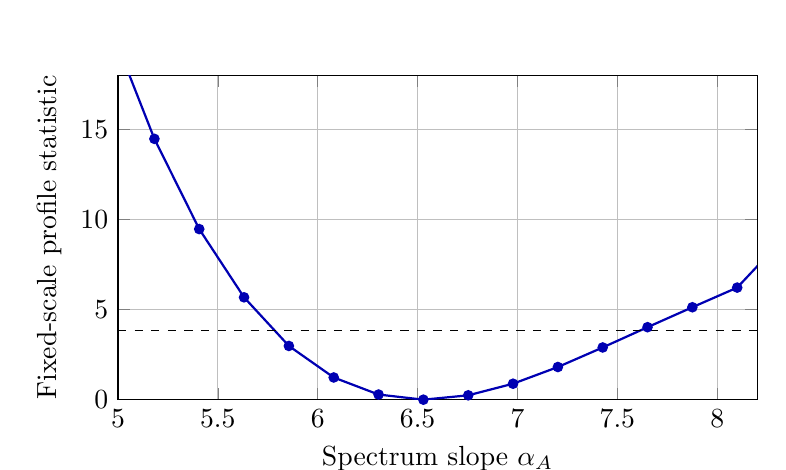
\begin{tikzpicture}
\begin{axis}[width=.8\linewidth,height=57mm,xlabel={Spectrum slope $\alpha_A$},ylabel={Fixed-scale profile statistic},
 xmin=5,xmax=8.2,ymin=0,ymax=18,grid=major]
% BEGIN GENERATED: profile_plot
\addplot[blue!70!black,mark=*,mark size=1.5pt,thick] coordinates {(3.1628121897031516,328.36384088809393) (3.3872160992337497,235.3783243436994) (3.611620008764348,159.80360707118547) (3.8360239182949467,102.84482765439618) (4.060427827825545,65.36145987547339) (4.284831737356144,47.6615857594127) (4.509235646886743,37.567945122328) (4.73363955641734,28.522264099323234) (4.95804346594794,20.810433277972706) (5.182447375478537,14.477629191992444) (5.406851285009136,9.4691600018038) (5.631255194539734,5.6807474416804284) (5.855659104070333,2.9824017869530572) (6.080063013600932,1.2322013674356211) (6.30446692313153,0.2852814511982099) (6.528870832662128,0.0) (6.753274742192727,0.24195906206549628) (6.977678651723326,0.8856750010230929) (7.202082561253923,1.812052804154736) (7.426486470784521,2.8981349458286676) (7.65089038031512,4.023087941456916) (7.875294289845719,5.130520545256355) (8.099698199376316,6.221263121313789) (8.324102108906915,8.867330397652474) (8.548506018437516,9.876382939944428) (8.772909927968113,10.702045106557202) (8.99731383749871,11.384410246164096) (9.22171774702931,11.947411292290061) (9.446121656559908,12.40927686809685) (9.670525566090507,12.78512288721646) (9.894929475621105,13.087980733132063)};
\addplot[black,dashed,domain=5:8.2] {3.841458820694124};
% END GENERATED: profile_plot
\end{axis}
\end{tikzpicture}
\caption{Central region of the original 31-point alpha profile, with all source coordinates embedded and the nominal threshold shown dashed. The original grid extends beyond the displayed range.}
\label{fig:profile}
\end{figure}

The bootstrap resamples calibration residuals independently within each training field, refits the spectrum, predicts the holdout field, and adds a draw from pooled calibration residuals. The recorded run retains \BootstrapCount{} converged refits. Its pointwise 95\% band has coverage \BootstrapCoverage{} and mean normalized-polarization width \BootstrapWidth{}. Complete coverage must be interpreted with the band width; it is not evidence of precise simultaneous coverage. The separate 1,500-draw holdout RMSE bootstrap is evaluation-only. Temporal correlation and model discrepancy are not included in these uncertainty constructions.

\section{Transport audits, refinement and migration evidence}\label{sec:verification}

\subsection{Frozen-generator invariants}

For a prescribed background, the generator audit checks column conservation, stationary residuals and
\begin{equation}
 \log(k_i^+/k_i^-)=-\beta(U_{i+1}-U_i),\qquad\beta=(k_BT)^{-1}.
\end{equation}
The reversible similarity transform is
$\mathrm{diag}(\pi)^{-1/2}Q\,\mathrm{diag}(\pi)^{1/2}$.
Tridiagonal eigensolvers compute its gap. The finite-mesh lower bound used in the native audit is
\begin{equation}
 \lambda_h\geq\frac{4D_{\min}}{h^2}\sin^2\!\left(\frac{\pi}{2N}\right)
 \exp[-\beta\,\mathrm{osc}(U)].
\end{equation}
At a positive, nonstationary probe, the entropy derivative is $(Qp)^T\log(p/\pi)$. Negative values check dissipation for the frozen generator. These checks do not establish nonlinear self-consistent stability or an upper occupancy bound under a biased linear probability propagator.

\subsection{Two different convergence experiments}

The \code{continuum} study fixes a representative occupancy of 0.30 only to choose a spatially constant diffusivity. It compares meshes $N=16,32,64,128,256$ against $N=512$ for the same constant-field exponential-rate law. Its reported order is fitted using $N\leq128$. The lower bound uses $D_{\rm eff}\pi^2/L^2\exp[-|E|L/(k_BT)]$ in the declared reference setting.

The \code{refinement} study follows the R3 notebook. It freezes either $c(y)=0.3+0.1\cos(2\pi y)$ or $c(y)=0.2+0.2y$, with $y=x/L$, retaining the full structure-dependent potential and edge diffusivity at each finite mesh. The reference sets only the mesh parity statistic to zero and uses 8,192 cells with a 4,096-cell doubling check. Time is $0.08L^2/D_{\rm rep}$. Modal propagation retains 128 modes, checks 256 modes on the reference, treats the known stationary component analytically, and is cross-checked against a matrix exponential at $N=64$.

For even $N$, the symmetric background has zero parity order up to roundoff, while the ramp has $m_{\pi,N}=1/(3N)$. A nonvanishing alternating profile, $c_i=0.3+0.05(-1)^i$, retains $Q_R=0.01$ \AA{} under refinement and does not represent samples of one smooth macroscopic profile. This limitation is deliberately visible in the code and output.

\begin{table}[htbp]\centering\small
\caption{Recorded convergence orders. The full-generator ramp exhibits first-order behavior and must not inherit the constant-$D$ second-order claim.}
\label{tab:orders}
% BEGIN GENERATED: orders_table
\begin{tabular}{lrr}
\toprule
Benchmark & All-grid order & Fine-grid order \\
\midrule
Constant $D$, field benchmark & 2.029076$^{a}$ & -- \\
Symmetric & 2.003088 & 2.007136 \\
Ramp & 1.001640 & 1.000370 \\
\bottomrule
\end{tabular}
% END GENERATED: orders_table
\par\smallskip\footnotesize $^a$For the constant-$D$ benchmark, the fit uses only $N=16,32,64,128$ against $N=512$; the R3 all-grid fit uses $N=16$ through 1,024 and the fine-grid fit uses its last four meshes.
\end{table}

\begin{figure}[htbp]\centering
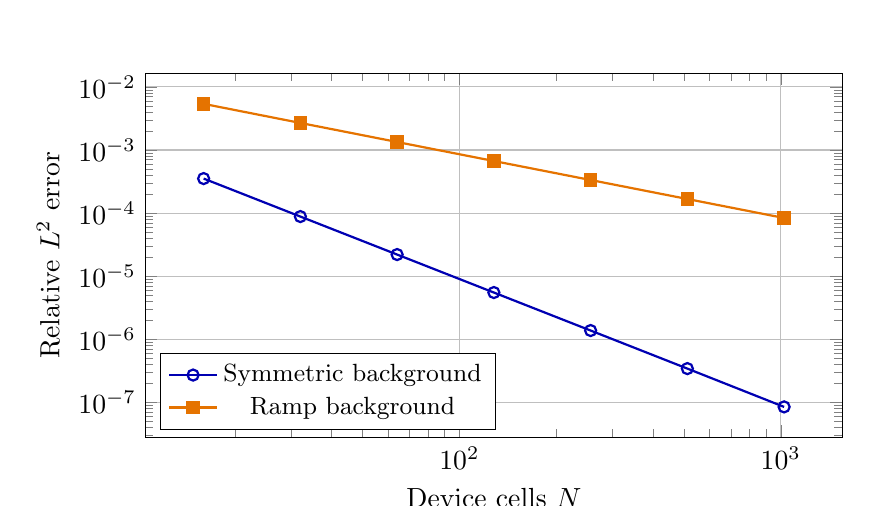
\begin{tikzpicture}
\begin{loglogaxis}[width=.86\linewidth,height=62mm,xlabel={Device cells $N$},ylabel={Relative $L^2$ error},
 grid=major,legend style={font=\small,at={(.02,.02)},anchor=south west}]
% BEGIN GENERATED: refinement_plot
\addplot[blue!70!black,mark=o,thick] coordinates {(16,0.0003521805951072897) (32,8.800331759233349e-05) (64,2.1991355714561715e-05) (128,5.496294192268485e-06) (256,1.3730350201004249e-06) (512,3.4225184944271227e-07) (1024,8.455805264130253e-08)};
\addlegendentry{Symmetric background}
\addplot[orange!90!black,mark=square*,thick] coordinates {(16,0.005385932829171535) (32,0.0026822524151361112) (64,0.0013384225306288468) (128,0.0006685818841964311) (256,0.0003341402635114154) (512,0.00016703329630447797) (1024,8.350751480855845e-05)};
\addlegendentry{Ramp background}
% END GENERATED: refinement_plot
\end{loglogaxis}
\end{tikzpicture}
\caption{Full-generator refinement against the smooth reference. Coordinates are embedded from the native R3 audit; finite meshes retain their original parity closure.}
\label{fig:refinement}
\end{figure}

\subsection{Independent coefficient sensitivity}

The transport sweep uses $\chi_A^{\rm tr}\in\{0,0.25,0.5,\chi_{\rm nominal},1,1.5,2\}$ with two uniform backgrounds and one nonuniform staggered background. Rates, stationary distributions, gaps and entropy derivatives are checked for each coefficient/profile pair. The interval $[0,2]$ is a conditional stress range, not an empirical confidence interval. No polarization refit is performed during this sweep.

\subsection{Three distinct verification layers}

The integration record contains three different counts: 24 package tests, the original \OriginalAuditPassed/80 notebook gates, and \MigrationChecks{} migration comparisons. They answer different questions. Unit tests check physical invariants and API behavior, including holdout isolation and the analytic Jacobian. Original gates reproduce the source notebook's implementation, consistency, validation and scope checks. Migration comparisons establish agreement between the restructured package and freshly executed source notebooks.

\begin{table}[htbp]\centering\small
\caption{Selected recorded migration comparisons. A comparison accepts $|a-b|\leq\mathrm{atol}+\mathrm{rtol}|b|$. The source JSON contains every comparison and its status. Scientific validation is not inferred merely from migration agreement.}
\label{tab:migration}
% BEGIN GENERATED: migration_table
\begin{tabular}{lrrr}
\toprule
Quantity & Max. abs. difference & Abs. tol. & Rel. tol. \\
\midrule
Primary holdout RMSE & 4.395e-10 & 2.0e-07 & 0.0e+00 \\
Constant-$D$ order & 9.442e-08 & 1.0e-05 & 0.0e+00 \\
Five profile endpoints & 7.198e-12 & 2.0e-06 & 0.0e+00 \\
Original alpha-profile SSE & 2.501e-07 & 1.0e-06 & 0.0e+00 \\
R3 relative $L^2$ errors & 2.848e-12 & 2.0e-10 & 2.0e-05 \\
R3 spectral gaps & 6.000e-15 & 2.0e-11 & 2.0e-07 \\
Sixteen retrospective RMSEs & 6.263e-10 & 2.0e-06 & 0.0e+00 \\
\bottomrule
\end{tabular}
% END GENERATED: migration_table
\end{table}

All four archived notebooks executed successfully in the recorded environment. All \MigrationChecks{} migration comparisons passed, including the 16 retrospective field/model scores and five additional profile intervals. This supports fidelity of the software migration. It does not add new material measurements or strengthen a physical inference beyond the source protocols.

The original reference summary also contains risk-AUC, transfer and hidden-twin results. They remain explicitly synthetic protocol results. Their historical variable names are preserved for provenance even where the current manuscript uses more restrictive terminology. The numerical file hash identifies the exact recorded result; the supplement does not assert bitwise identity of every synthetic downstream scalar with every printed manuscript decimal across numerical environments.

\section{Reproduction, documentation and artifact lifecycle}\label{sec:reproduction}

\subsection{Environment and commands}

The project declares Python $\geq3.12,<4.0$ and uses Poetry with a checked-in lock file. The recorded numerical environment is Python \RecordedPython, NumPy \RecordedNumpy{} and SciPy \RecordedScipy. The installed package version is \PackageVersion. This is a source/evidence snapshot of the working tree, not an assertion that the changes already exist in a tagged public release.

From a complete repository checkout, the minimal and full protocols are:
\begin{lstlisting}
poetry install
poetry run proton-study --study calibration
poetry run pytest -q

poetry run proton-study --study all --output paper_results
poetry run proton-reference --output reference_results
poetry run python scripts/verify_migration.py \
  --native paper_results --reference reference_results \
  --output validation/migration.json
\end{lstlisting}

The nine native study names are \code{calibration}, \code{review}, \code{uncertainty}, \code{identifiability}, \code{transport_sensitivity}, \code{continuum}, \code{refinement}, \code{hidden_state} and \code{start_sensitivity}. Their separation prevents retrospective scores or conditional transport tests from being confused with the primary holdout.

The default bootstrap has 100 refits. The source seed is 20260802 and the calibration bootstrap uses seed 20261503. Reducing \code{--bootstrap-repetitions}, enabling \code{--original-profile-only}, or changing \code{--reference-cells} changes the numerical protocol and must be recorded as such. The reference runner accepts one original notebook filename and a per-cell timeout, defaulting to 3,600 seconds.

\subsection{Outputs and reproducibility identity}

Each native study writes named CSV tables, JSON metadata and environment versions, optional compressed arrays, and available vector figures. A manifest hashes the rendered artifacts. Original notebook replay writes executed copies in separate directories, a success/runtime/interpreter record, and notebook-specific outputs. Scientific execution uses the embedded data after dependency installation and does not redownload the original publisher workbook.

Numerical comparisons use declared tolerances because optimizer, eigensolver and BLAS variations can alter final digits. Compressed archive and PDF bytes may also differ across builds without a numerical difference. SHA-256 identity of source notebooks or numerical input bytes serves a different purpose from tolerance-based agreement of recomputed results.

\subsection{Sphinx, Google docstrings and Pages}

Code documentation is written in English using Google-style class, constructor and method docstrings, including units and scientific scope. Sphinx autodoc and Napoleon render the API, while Mermaid diagrams describe architecture and execution. The build command is
\begin{lstlisting}
poetry run sphinx-build -b html -W --keep-going \
  docs/source docs/_build/html
\end{lstlisting}

The documentation workflow runs tests and builds Sphinx before eligible default-branch deployment through GitHub Pages artifacts. It is prepared in the repository; local compilation does not imply that a remote deployment has taken place. Historical generated HTML outside the workflow output is not the current publication source. The separate manual reproduction workflow runs the complete native and notebook campaigns and their migration comparison.

\subsection{Single-file supplementary document}

To use Overleaf, upload only \repo{supplementary/main.tex} and select pdfLaTeX. The file contains all prose, tables, bibliography entries, TikZ diagrams and PGFPlots coordinates. No external image, CSV, JSON, bibliography file, shell escape, or auxiliary source directory is required for compilation. The embedded plot values are recorded model outputs rather than calculations executed by TeX.

Repository maintainers can refresh only the named evidence blocks and build locally:
\begin{lstlisting}
poetry run python scripts/update_supplement.py
poetry run python scripts/build_supplement.py
# Preserve all existing inline content without refreshing evidence:
poetry run python scripts/build_supplement.py --no-refresh
\end{lstlisting}

The updater verifies notebook and artifact manifests before embedding values. It changes only blocks delimited by \code{BEGIN GENERATED} and \code{END GENERATED}, preserving manually edited narrative. The local builder copies the single file into an otherwise empty temporary directory and runs pdfLaTeX there. Successful isolated compilation therefore also checks that hidden repository dependencies have not been introduced. Intermediate TeX products are temporary; the finished PDF is written alongside the source.

\section{Source provenance and limits of interpretation}\label{sec:provenance}

\subsection{Original notebooks and experimental matrix}

The complete original notebook sources~\cite{notebooks} are preserved byte for byte. Their individual identifiers are:

% BEGIN GENERATED: notebook_hashes
\noindent\textbf{\path{Hx_NdNiO3_single_cell_evidence_calibrated_PoC_v3_1.ipynb}}\\
{\small\path{3929eb8def57f4f883706baf2a099b7ad13c8fd6d6bf6cd793ff83afa03640ad}}\par\medskip
\noindent\textbf{\path{proton_R2_5_identifiability.ipynb}}\\
{\small\path{590e161eddac4f0d22734fc005944849669bcc3a3159e17114463c64958fadca}}\par\medskip
\noindent\textbf{\path{proton_R3_full_generator_audit.ipynb}}\\
{\small\path{db78d07c30a2ef7b03939ba3e3133afabaae33b1fc57a3d280da02c62b3d261e}}\par\medskip
\noindent\textbf{\path{proton_review_addendum.ipynb}}\\
{\small\path{9159a6cb9f9300b7e731c12ecaf096650e5a1fcd40bec90aba729f3a92077a9c}}\par\medskip
% END GENERATED: notebook_hashes

The numeric experimental matrix checksum is
\begin{quote}\small\path{859f76869eb087bc05e0aba24f3543bddb90b03842d10bb49d0dc66d1814354a}\end{quote}
This hash refers to contiguous little-endian float64 matrix bytes, not to JSON file formatting. The inherited publisher workbook hash is
\begin{quote}\small\path{e8e7933e8648b49d115f6f20bb1752cce54c078dfdd21b3a8d433671043f5f2d}\end{quote}
The original workbook is not bundled; retaining its source-record hash does not claim an independent re-extraction during integration.

\subsection{Manuscript and implementation identity}

The supplied \code{Proton_T.pdf} is identified by SHA-256:
\begin{quote}\small\expandafter\path\expandafter{\PaperHash}\end{quote}
The source/evidence snapshot used to generate this document is identified by:
\begin{quote}\small\expandafter\path\expandafter{\SnapshotHash}\end{quote}
The full JSON snapshot is embedded as comments at the end of this source file, including individual source/evidence hashes and the base Git commit. Its digest is computed from the indented JSON text with a final newline before comment prefixes are added. The snapshot excludes this \texttt{.tex} file itself to avoid a circular checksum. A base commit identifies ancestry only: it must not be cited as though it contains uncommitted implementation changes. A final publication release can add a stable tag or archived DOI after the reviewed repository state has been published~\cite{repository}.

\subsection{What alignment does and does not establish}

The current implementation and original reference workflow support the manuscript's modular interpretation: literature-constrained structural transport, separately evaluated polarization relaxation, and diagnostic information loss. The historical engines remain outside that interpretation. The following boundaries apply to both software usage and the wording of resulting publications:
\begin{itemize}
\item The retained structural subspace and one-dimensional coarse mesh are reduced descriptions; they are not a full crystal or an independent many-electron simulation.
\item The parity statistic is a mesh-defined proxy. The observed first-order ramp behavior is retained as a limitation rather than hidden by a universal second-order claim.
\item Frozen-generator conservation, detailed balance and entropy checks do not prove stability of a general nonlinear evolving-occupancy problem.
\item The relaxation law is independent of transport trajectories. Its holdout validates the declared prediction task, not a unique dynamical concentration-to-polarization mechanism.
\item Coefficient transfer, fixed-scale profiles and pointwise residual bootstrap retain their conditional assumptions. Finite intervals are not independent identification of microscopic constants.
\item Risk and hidden-twin experiments are synthetic protocol studies. The native reflected-pair illustration does not reproduce their entire experimental-design procedure.
\item Unit tests, the original 80-gate record and migration comparisons establish different forms of computational evidence; none is a new physical experiment.
\end{itemize}

\begin{thebibliography}{9}
\bibitem{manuscript}
J.~Villalba-D\'iez, A.~Bello-Garc\'ia and J.~Ordieres-Mer\'e,
\emph{Proton Transport and Polarization Relaxation in \material: Literature-Constrained Reduced Models and a Recoverability Diagnostic}.
Supplied manuscript, \code{Proton_T.pdf}, identified by the checksum in this supplement. No publication DOI is assigned here.
\bibitem{yuan}
Y.~Yuan, M.~Kotiuga, T.~J.~Park et al.,
``Hydrogen-induced tunable remanent polarization in a perovskite nickelate,''
\emph{Nature Communications} \textbf{15}, 4717 (2024).
\url{https://doi.org/10.1038/s41467-024-49213-0}.
\bibitem{lione}
A.~Lione, J.~\'I\~niguez-Gonz\'alez and N.~C.~Bristowe,
``First principles study of [111]-oriented epitaxially strained rare-earth nickelate NdNiO$_3$,''
\emph{Physical Review B} \textbf{113}, 014119 (2026).
Literature input cited by the supplied manuscript and notebook record.
\url{https://doi.org/10.1103/k48x-mvw1}.
\bibitem{repository}
QC-UPM, \emph{OgTRQC repository}.
\url{https://github.com/QC-UPM/OgTRQC}.
This document describes local package version \PackageVersion{} and the embedded source snapshot, not an asserted tagged public release.
\bibitem{notebooks}
\emph{Original computational record for the proton-transport manuscript}.
Four supplied notebooks: v3.1 evidence-calibrated proof of concept, review addendum, R2.5 identifiability diagnostics, and R3 full-generator audit. Archived under \repo{notebooks/reference/}; checksums are listed above.
\end{thebibliography}

% The complete input snapshot is a comment block, not an external build dependency.
% BEGIN GENERATED: source_snapshot
% {
%   "package_version": "0.2.0",
%   "base_git_commit": "9df09a4b999b9ce6d918c57f19c6aea45a84ec51",
%   "identity": "Source/evidence working-tree snapshot; the base commit is not a release identifier for uncommitted changes.",
%   "source_files": {
%     "VARIANTS.md": "3e5a46b6ff8876bd86a5a752aa0cd46f3050a446134d8d35d22613c987f49937",
%     "notebooks/reference/Hx_NdNiO3_single_cell_evidence_calibrated_PoC_v3_1.ipynb": "3929eb8def57f4f883706baf2a099b7ad13c8fd6d6bf6cd793ff83afa03640ad",
%     "notebooks/reference/manifest.json": "17ba5546a120d50ca6a2b9a1150ee79ae767a8ba33e84d11b07b92bbf5c4554c",
%     "notebooks/reference/proton_R2_5_identifiability.ipynb": "590e161eddac4f0d22734fc005944849669bcc3a3159e17114463c64958fadca",
%     "notebooks/reference/proton_R3_full_generator_audit.ipynb": "db78d07c30a2ef7b03939ba3e3133afabaae33b1fc57a3d280da02c62b3d261e",
%     "notebooks/reference/proton_review_addendum.ipynb": "9159a6cb9f9300b7e731c12ecaf096650e5a1fcd40bec90aba729f3a92077a9c",
%     "octa_gtrqc_sim/proton/__init__.py": "39ca57fb19933e780e3bb66d4f8dee6dc08a6b3f872f92710ec519dcdb5c3b81",
%     "octa_gtrqc_sim/proton/audits.py": "551a9b0b14344f2e6d4885bc4c28a03640acaee13fe11fd26e22783ed3af346d",
%     "octa_gtrqc_sim/proton/cli.py": "408292fb1d78b3e29809fd8195118839faa304a26c591a0a5bd9a5280c3ca712",
%     "octa_gtrqc_sim/proton/data/fig2h.json": "8c2443cbd25cce947f2cae4738862af6ba096daf40cfc2f29edcd4a3cf8c8dc3",
%     "octa_gtrqc_sim/proton/data/provenance.json": "0ccc99c089801a1966e8c6e186c30db346fd67012226abb8fda2367d58bbe97d",
%     "octa_gtrqc_sim/proton/dataset.py": "7d4dc4580c5f54d4792119422863655bf93c97ddd3296153ae5ebe2979aeac65",
%     "octa_gtrqc_sim/proton/diagnostics.py": "3e3917c3b024bee34221ce23b4f19ebf072ae48016d84efd3020d39014641724",
%     "octa_gtrqc_sim/proton/identifiability.py": "7835b87a2540bdd7a14d741d7a489629cc2cd39101458673c7a89d6026312bbe",
%     "octa_gtrqc_sim/proton/presentation.py": "3264db0eef2ba64b79000f2bd94335e17f9ba2cc26845d5caa67a41f4bfe1cad",
%     "octa_gtrqc_sim/proton/reference.py": "aa32aaaebe8834871dd304a1ca2dd48f8d67cf2a019c40e0f4c84db6b591b592",
%     "octa_gtrqc_sim/proton/relaxation.py": "5e3e7a74cd2bc514a6322a8fe1a45a94c88819e1bf01ce839aefe03a26a1a20a",
%     "octa_gtrqc_sim/proton/structure.py": "6f7538381ccd80175ba0607d8d509f498f625a89762151af2aaad8d1bbd8b1ae",
%     "octa_gtrqc_sim/proton/studies.py": "c870d6f5b11be6ad58866625c249630d44b43d88c9108bb81c064f2111eedb95",
%     "octa_gtrqc_sim/proton/transport.py": "d3db69456c40d972ab758a7c6cd56d4f21bc5ef724262cc45e9f247f8fa3d4c2",
%     "poetry.lock": "2b96db15413a98adb592ded6629e12dc3418b800f2c5616fad9b4162d22d8dc1",
%     "pyproject.toml": "6e8b5e3a7fef9aa30459799d7bd5e8ff1b8fb63d4849434c601b60a43539f0c1",
%     "scripts/build_supplement.py": "324233836308bf6e03c59e35d7cb22ae0984580a3c2a9f33cc3b766594db4b24",
%     "scripts/update_supplement.py": "450da1a722645f27e1ef97f64e5671f864b711d767aff02c99ebef4e3c915dbb",
%     "scripts/verify_migration.py": "c4449d5d4e19c0b4bcf164e8bc4a320a77ec0c88fbe91c1a2af56a4d23173109",
%     "tests/conftest.py": "a10507c92b5fd1647a3fb2551344077bbc7909eb47d690a2d3dcc78db0770e84",
%     "tests/test_proton_models.py": "6b90d841b41c027cab98c28b6bfde8c33f75f5e8156a6675e147fae5e760bd37",
%     "tests/test_robustness.py": "100fb2e59f640e475819017812a656eef4f68011d1672a7423dbccb935f92977",
%     "validation/migration.json": "7264e958b8ab180a3d55c98e80acfeff4f0fbee114a05017ea82f87387f99cbb",
%     "validation/native/calibration/README.md": "254b2b483e82892b81c8976c73de983bd8df3de9bee2ae8dd6b898546019cec2",
%     "validation/native/calibration/figure.pdf": "8da36e83b1c01dfc419296239e9fb9d3a807e466c7267bd274a27eebf9a416ab",
%     "validation/native/calibration/figure.svg": "6bce0f18428f6cca2a50a296099bbdc536ec07268375802db78058ad20438d07",
%     "validation/native/calibration/information_criteria.csv": "13ca3a3aae941bc529ac4ee9f080de4064c17bdff4f0999a444acdaa2afa7d31",
%     "validation/native/calibration/manifest.json": "0d94b391cb9a5f3f8c5c0bca6b11d36c833aa5c28ede60096bd77a10e682a2bf",
%     "validation/native/calibration/metadata.json": "f12e9e0ea78b30e1d84df5b41b28a1649f26d7f84c9e5cfdcad40d6c38c5ba09",
%     "validation/native/calibration/predictions.csv": "c7b9d41642cdab8006392f2390fbb55e9e57f49a2cd497751cc54fc9fd471be5",
%     "validation/native/calibration/scores.csv": "638514fecad3f5ae9d1a6bee4898ea1914fe55b2da9587469a6533528857e002",
%     "validation/native/continuum/README.md": "4954926410f20d42780867c8c845494569a86fa72d63c86543afac2fbbfef3bf",
%     "validation/native/continuum/convergence.csv": "f2b2c079b9ed69773b5fc2170865860758c3470628dac491d1c9ac17f4adb5b6",
%     "validation/native/continuum/manifest.json": "569f21ca160dd6ad69a9ecc544cc20cfeb278dc0b9fb97e29cd75c337d558b26",
%     "validation/native/continuum/metadata.json": "635dddfe85fb028ca49cc9c973f33400f6ad3ae79d49fa93794aabeead0ff8fd",
%     "validation/native/hidden_state/README.md": "7db708b05f11dd29685413d7774f70dbc46e415be82861bc7aa3dcf0be9fba3b",
%     "validation/native/hidden_state/manifest.json": "a10b5e6f293890c5cd93f581115430e91f1c1832b3ab9675ff4f0538ef5965f8",
%     "validation/native/hidden_state/metadata.json": "340a68433b2460eedaecc2612a81b678471eb81d34f04e4c142b74b88be405eb",
%     "validation/native/hidden_state/reflected_pair.csv": "f71aea872527ec72bf26028e78d358251d0ba5963ba32a5b4b130d3ab219cee1",
%     "validation/native/identifiability/README.md": "8eb1fe54e20417f83ee6d130846d390378d4c0c03b2f1994e05f0eb339d574f6",
%     "validation/native/identifiability/additional_profile_intervals.csv": "c03c80282aa5ee49c0d353f2ed9782354d462081968a5b5df1cf6549204d3d7e",
%     "validation/native/identifiability/figure.pdf": "956776b4d769a551b385edcd3fee27dd05fcf03864c9d2b8b848ab4b277eb012",
%     "validation/native/identifiability/figure.svg": "da5652e09850c76a63be261630d1b87d63b840e3416fcfb4b3e3bdada729278a",
%     "validation/native/identifiability/manifest.json": "88c15c65004523d33224dd38b040cc61763bd77ac8d85c38ae707fe4013d9362",
%     "validation/native/identifiability/metadata.json": "ec4889a1262d3334d17c41eb3ea543b77f17fda389e0bbc8e3da092846947dda",
%     "validation/native/identifiability/original_alpha_profile_31_points.csv": "a9f3054cc2b146d573be2acfaea9bfe7498e4be6cd29325ad830b082b6eb6dec",
%     "validation/native/identifiability/parameter_correlation.csv": "10ed28c742a147afb4ce15d5577737491675910ea2ba54471fd86b2da5079db3",
%     "validation/native/identifiability/profile_b0.csv": "27ed57711b81ed18731e7d53a6b9f4b85b7daab4d32c0021ee01b2f93084f0e8",
%     "validation/native/identifiability/profile_b1.csv": "17bed8ac0bec663c5b4b7c7d0c11e875689fb4e706b9e6d508dda562ecf90a14",
%     "validation/native/identifiability/profile_b2.csv": "710a7c7f750d1a1097708c22e22794aadc18c815a74db01d656a5345df61bbdc",
%     "validation/native/identifiability/profile_cF.csv": "423bf2b1b7dc0bde8b82c571878c825f1c5bbce6d8180db77824d2cf1597e461",
%     "validation/native/identifiability/profile_log_tau0.csv": "b52253a0ec95f35bf641766fd0008999db33ee0dab0447f45c3396c51d486148",
%     "validation/native/refinement/README.md": "2f3f22589eb8851a7ab7d33d74c495810969215a7dc601865dadd2c39029d235",
%     "validation/native/refinement/arrays.npz": "8ca6569f824b185443ffedd7714f3c4b45bedf56ed6b1d263bcc34f246aa89b6",
%     "validation/native/refinement/figure.pdf": "cc034dddf1517d24731ed03bdf7d2160017c19c08848fea2dd00463865c0c8f5",
%     "validation/native/refinement/figure.svg": "e893947465479115385f8d48a7fdf51f22966fc0919f8fa08856e194d01b74f9",
%     "validation/native/refinement/full_generator.csv": "2e5de33cb12032c2e6b69f250b9bebb8ade977e3f57bf839e9cab217ee226ffe",
%     "validation/native/refinement/grid_alternating_counterexample.csv": "996a1e29f44d401a87c822489829a3acf4eb1fcd595b1bc22041e020085c40ba",
%     "validation/native/refinement/manifest.json": "73d4db518c7fde66704aa844c87899f79bae83da3954adbcae3db583f192a304",
%     "validation/native/refinement/metadata.json": "681b5783772ab8fc1cedb4f5382cd26d44fcec1e242ca757b7247961679a6a33",
%     "validation/native/refinement/orders.csv": "bda27ae82971b27a8dc5655d004b5023d015b0cb0cedc20477b189885706142b",
%     "validation/native/review/README.md": "39741ee817ae7733944f1fb460b5a83e1b1a1759857c3c77d4e23b9b7b7ce617",
%     "validation/native/review/figure.pdf": "29cb8fe9d4c9b37ee959b5845f37b95e0c29db23a9315f0cea1a6e6a8f8fa8e6",
%     "validation/native/review/figure.svg": "5a1b4ff64d5aa07ca1883944a2ef9268067cec7ba500a7b9193cbbe972bb9358",
%     "validation/native/review/information_criteria.csv": "de34b2e40c76312320886f25931fd5f7f9003ee02f83eacbafe7aa0f984dca5d",
%     "validation/native/review/manifest.json": "b269b449dfc17eb391aecaaae6c22f291c39a5277ec0cf80e4d10173b3012952",
%     "validation/native/review/metadata.json": "9d92a95dac6c3e55777c4f873611c670245029d1c2833f690cd405ab191d74dd",
%     "validation/native/review/predictions.csv": "288cee74b286516213fb51a94c364dcb4aaed7409d3a79a21858e74c0d67a919",
%     "validation/native/review/scores.csv": "3e7fd253a06197cc89e63ba4bdb7a54f04bf49335caffe32b9bf27b843a3d64e",
%     "validation/native/start_sensitivity/README.md": "56a277403d895fcab9c610c25b4a3cb694cf987091c10090597052437fff6020",
%     "validation/native/start_sensitivity/audit.csv": "bbd8dbdc3d652c94ae29081b33b44220cc37feaec75984c5a20dc57851ad9235",
%     "validation/native/start_sensitivity/manifest.json": "6d5caed684b1df73726e5e8be78fe36d37c76c24dd3f24661710315185a1beca",
%     "validation/native/start_sensitivity/metadata.json": "b4bd9c706f6194b38c003433e92bab25ed084649dd8ea506ff1edea1ea876e81",
%     "validation/native/transport_sensitivity/README.md": "5f21014a39fe879832c0c5e4bd0bd12f706fdb114966b3c475f32e84915072be",
%     "validation/native/transport_sensitivity/frozen_generators.csv": "95d96a348df209d03fe3b5c9acd2dc04babc01d2d6f4d0023d1ecdbe91be5c47",
%     "validation/native/transport_sensitivity/manifest.json": "9a6cee0073ba0eaac94adff7e6ba68bf85f2ab673a3f3685505ae701442c2400",
%     "validation/native/transport_sensitivity/metadata.json": "6479b7892f37ed96b24ecf3ae07ab4f434011bf1bea76384f847a7863ba4838b",
%     "validation/native/transport_sensitivity/sensitivity.csv": "d2390deb7c151a6200e67a46d3cc5cbd538f9e83ddd5402b6fc3f2c7fa2547d3",
%     "validation/native/uncertainty/README.md": "fe9f2fbd0b6b48a1919f5aad05ae4f4c58bfb8c768cbc157cbc028d1be93854c",
%     "validation/native/uncertainty/arrays.npz": "0061f65cb54ade64e871048c4ce9154afe0c33e4fbf775df3c50a9779fa7e269",
%     "validation/native/uncertainty/figure.pdf": "78fe56eace081a858adaad56ea981ef8210ffe38ac0226efdd8a82528fec9a9c",
%     "validation/native/uncertainty/figure.svg": "e0e7305d4a0c5bc3444c6965b4e32bde119e12de047ae97354fb5b889f389521",
%     "validation/native/uncertainty/manifest.json": "10fadf3e86e0697984fd93b21378c94c46d4eaf48608f41150244a38e732dbb0",
%     "validation/native/uncertainty/metadata.json": "f60fb78386c61f429e2b61827b387adfc2ad8e0fcb76fa4c4523221b59f6a750",
%     "validation/native/uncertainty/prediction_intervals.csv": "c5f555fa62d14be43c234dd767ed3d03f76f1fd55cedffd0ff7fea99595beebe",
%     "validation/reference/Hx_NdNiO3_single_cell_evidence_calibrated_PoC_v3_1/execution.json": "445924f098d0445619f2cabca8ef917b2cef2f1137e68c6dd4b5034c1d7331da",
%     "validation/reference/identifiability/interval_b0.json": "c1e5c0a11488264d96951184c5229e9c321d1976e450bf1172aea1aae2b47b22",
%     "validation/reference/identifiability/interval_b1.json": "ba13b05d18f84a82a8d4ec2e90186125626c1609d507e509b2f3b3eac0d2dd4e",
%     "validation/reference/identifiability/interval_b2.json": "f5899f6aae2445867b76deaf3e6545b639505cd5ba6fab43cb085d4f4da57890",
%     "validation/reference/identifiability/interval_cF.json": "e8a3a2b7fd4a1cdffcad6da64c7e924a7c24e4cc1112e8f243fc3edc63e2194b",
%     "validation/reference/identifiability/interval_log_tau0.json": "699911841d50296ee6d890bc06d1d56895fc040991deacc378555b35aa2bff6c",
%     "validation/reference/identifiability/provenance.json": "7cf5249130fd7d70527aa7a43f32d06572e9f1aa71bb16621f2053ee87cb883e",
%     "validation/reference/identifiability/revision_checks.json": "54035770009a70af970eb0f4a9a8b6b07905aaeedfe7c9f62a8c5e027f47f47a",
%     "validation/reference/proton_R2_5_identifiability/execution.json": "1c46b55ec4d448f8c839aa7f87504798043ce674eb97ff4ef0b83289711b5bff",
%     "validation/reference/proton_R3_full_generator_audit/execution.json": "4592fddac0966ec2e58b8ca2c30949587c3b49d5f1f7020e02a021d52de2d855",
%     "validation/reference/proton_review_addendum/execution.json": "836a989d0797c5b9d0163b6b00f2e926eb216c062c4b818540e8b9c744f7d195",
%     "validation/reference/refinement/numerical_checks.json": "b7135f24aa8f1a7c0786c010e182ff4895e4b8a4e70b4edd5e4b23226aaa1bbd",
%     "validation/reference/refinement/summary.json": "01823d3805dfc1e8bbfb3ca857fd2464a7a079e0f6a5650c66898ef4944923af",
%     "validation/reference/review/biexponential_start_audit.json": "1e246ae27144c02bbf25571931e15282cf2242a76a1b871a7c50d6beaf19541a",
%     "validation/reference/review/fit_parameters.json": "d1933fe54ce0d69a75f39546e816b99bd95c943d0774303751e900ab53075168",
%     "validation/reference/review/original_model_start_audit.json": "c2faf797f551979ef59bc24bfb6c675b029a94f9083f4e5797aad9697b15a0a2",
%     "validation/reference/review/provenance.json": "ea70656ecdd7a3ed3ae76df68e07958552c370d501164d9de98a272ed5839069",
%     "validation/reference/review/revision_checks.json": "ea76d62551656d8143e5c819b5faff50c99c425f95ddb4eec8a6ffd7e8ed1dec",
%     "validation/reference/summary.json": "9a38e0eee7fba5172b418240b20dfa57d3e6d45c05e4b2bb476fe73cbe2c269a"
%   },
%   "supplied_manuscript_sha256": "30fcc98b7d9191c0f5b5fe909b817d09138dddafb0877010853901daf25126fd"
% }
% END GENERATED: source_snapshot
\end{document}
